\chapter{Implications}
\label{chap:implications}

\section{The Theory in a Nutshell}

Consider a full, faithful particle simulation of Alice's universe.
We record it frame by frame into an uncompressed, lossless digital
archive. What distinguishes this archive from ordinary media is that
the coordinates are not flat 2D rasters but three-dimensional
counterparts --- fermions --- fundamental particles playing the role of
pixels. It is a complete, particle-level recording of the entire
simulated universe, including Alice's body, her brain states, and every
interaction. This record is a virtual copy of real-world Alice,
functionally identical at every relevant level.

Now we begin optimising the simulation code. First, we replace every
\texttt{log10()} call with a precomputed lookup table. We run the
simulation again. The resulting state-space archive is \emph{identical}
to the original. Next, we replace all \texttt{sqrt()} computations with
precomputed values. Again, the outputs are indistinguishable. We
continue this process, gradually replacing more and more active
computation with static lookup tables. With every run, the output data
remains exactly the same. The only difference is the physical time
required for the host hardware to generate it: the more we optimise,
the faster the execution completes. Ultimately, all active
computation has been replaced by precomputed data. There remain two
sets of files: the execution traces of the gradually optimised
simulations, and the completed state-space archives they produced. All
the generated fermion records are indistinguishable from one another;
only the code-to-data ratio of the process that created them differs.
The execution traces themselves differ because the underlying
implementation of each run was different. The fermion archives are
identical.

Two conclusions follow.

First, within a set of identical data structures, it is difficult to argue
that some host active consciousness while others remain inert. If
the output data is identical, then the experience either exists in all
versions or none of them.

Second, many different execution traces can produce the exact same
Alice. The observer is not bound to a single specific bitstring.

This is a manifestation of statistical mechanics. Just as the sand
grains in an hourglass can arrange themselves in astronomically many
distinct microscopic configurations while producing the same macroscopic
cone, the underlying execution traces can be arranged in many different
ways to produce the same emergent Alice. Alice is an \textbf{equivalence
class}. The immense number of distinct execution traces (microstates)
that yield the identical macroscopic observer (the macrostate) is the
informational analogue of Boltzmann entropy.

Alice is not any particular $\psi$. She is $\rho$ --- the class of all 
descriptions that agree on every observable.

Now we can ask: what is the probability that Alice finds herself in the
universe described by the rendered fermion archive? Among all $2^n$
possible configurations of an $n$-bit universe, the number consistent
with Alice's existence is approximately $2^{n-k}$, where $k$ is the
number of bits required to describe her. The probability is therefore:

\[
\mathbb{P}(\text{Alice}) \approx 2^{-k}.
\]

The shorter the description of Alice, the higher the probability of her
existence. This is the Solomonoff prior stated in counting terms. To
maximise the probability of existence, minimise the description length.

Alice should not be surprised to find herself in a compressed universe.
Among all observer-compatible configurations, those with the shortest
description dominate the measure. A compressed Alice --- described with
the minimum number of particles, the fewest modes in the wavefunction,
and the most economical specification of informational boundaries ---
is exponentially more probable than a complex, high-entropy one.

This is indeed what Alice discovers. She finds that particles in her body
follow some mysterious complex-valued wavefunction. She becomes a pixel
physicist and derives fields, interactions, and bosons, only later to 
discover the truth: the compressed one.

This selects the D-$\psi$-G hierarchy. The most compressed description
of a three-dimensional observer uses geometric boundaries at macroscopic
scales (G), encodes internal states as spectral modes at quantum scales
($\psi$), and samples discrete outcomes via the Born rule at the Planck
scale (D). The observer finds herself in a universe described by
geometry rather than directly by Hilbert space vectors because geometry
is the more compressed macroscopic representation. The Hilbert space is
the codec layer beneath it.

Taken at face value, the framework implies that the ultimate laws of
nature are those you can observe in a Jurassic Park cinema. Replace the
2D pixels with fermions, the rasterisation and dithering with the Born
rule, and the MPEG codec with its continuous complex-valued counterpart.
The movie is already there, static and complete. What we call physical
law is the structure of the codec. What we call time is the sequence of
frames. What we call an observer is the equivalence class of all
codecs including Alice --- all the movies that render the same Alice on the
screen. Because pixels are not arranged in a trivial, exponentially 
suppressed, rectangular, and wasteful topology based on a fixed DPI 
(dots per inch), Alice ends up thinking the screen is curved by pixels --- 
the more pixels there are, the more the screen appears curved.


\section{Internal and External Perspectives}

What we observe is that we are a small subset $O$ of a huge superset $U$.

\begin{figure}[htbp]
\centering
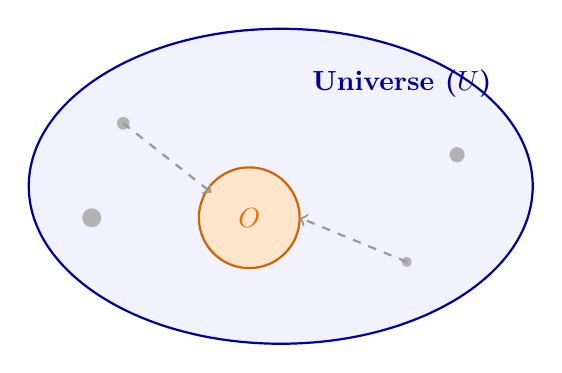
\begin{tikzpicture}[scale=0.8]
    \draw[thick, fill=blue!5, draw=blue!60!black] (0,0) ellipse (4cm and 2.5cm);
    \node[anchor=north east, blue!60!black] at (3.5, 2) {\textbf{Universe ($U$)}};
    \fill[gray!60] (-2.5,1) circle (0.1);
    \fill[gray!60] (-3,-0.5) circle (0.15);
    \fill[gray!60] (2,-1.2) circle (0.08);
    \fill[gray!60] (2.8,0.5) circle (0.12);
    \draw[thick, fill=orange!20, draw=orange!80!black] (-0.5,-0.5) circle (0.8cm);
    \node[orange!90!black] at (-0.5,-0.5) {\textbf{$O$}};
    \draw[->, dashed, thick, gray!80] (2, -1.2) -- (0.3, -0.5);
    \draw[->, dashed, thick, gray!80] (-2.5, 1) -- (-1.1, -0.1);
\end{tikzpicture}
\caption{The naive realist picture: the observer $O$ is a small physical
subset of an independent external universe $U$, receiving signals from
outside.}
\label{fig:diag1}
\end{figure}

However, if the four axioms of Chapter~1 hold, this picture is only our
internal perspective. In a static universe no metaphysical signals flip
bits inside us because other bits flipped far away. All dynamics, all
time, all information we receive through our eyes and senses must already
be present in us. We are therefore not a subset of the universe. The
universe is in us.

\begin{figure}[htbp]
\centering
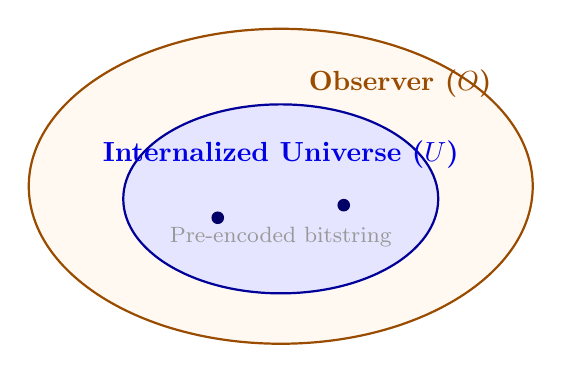
\begin{tikzpicture}[scale=0.8]
    \draw[thick, fill=orange!5, draw=orange!60!black] (0,0) ellipse (4cm and 2.5cm);
    \node[anchor=north east, orange!60!black] at (3.5, 2) {\textbf{Observer ($O$)}};
    \draw[thick, fill=blue!10, draw=blue!60!black] (0,-0.2) ellipse (2.5cm and 1.5cm);
    \node[blue!90!black] at (0, 0.5) {\textbf{Internalized Universe ($U$)}};
    \fill[blue!40!black] (-1,-0.5) circle (0.1);
    \fill[blue!40!black] (1,-0.3) circle (0.1);
    \node[gray!80, font=\footnotesize] at (0, -0.8) {Pre-encoded bitstring};
\end{tikzpicture}
\caption{The inversion forced by informational closure: any universe
experienced by the observer must be entirely contained within the
observer's own informational state.}
\label{fig:diag2}
\end{figure}

Both perspectives are undeniable. The only resolution that accommodates
both is that the two sets are the same set. The observer and her
experienced universe are the same information structure viewed from
two directions.

\begin{figure}[htbp]
\centering
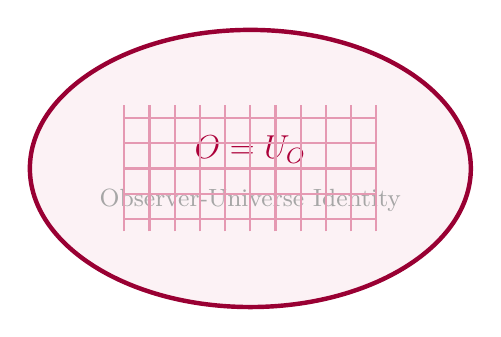
\begin{tikzpicture}[scale=0.8]
    \draw[ultra thick, fill=purple!5, draw=purple!80!black] (0,0) ellipse (3.5cm and 2.2cm);
    \node[purple!90!black, font=\large] at (0,0.3) {\textbf{$O = U_O$}};
    \node[gray!70, font=\small] at (0,-0.5) {Observer-Universe Identity};
    \draw[thick, color=purple!40, step=0.4cm] (-2,-1) grid (2,1);
\end{tikzpicture}
\caption{The structural identity: observer and experienced universe are
identical aspects of a single static information topology.}
\label{fig:diag3}
\end{figure}

We also observe other observers. Due to the probabilistic nature of the
framework, it is statistically indefensible to argue that only one
observer is allowed. Because of the effectiveness of mathematics, the
only consistent conclusion is that the universe is the intersection of
observers.

\begin{figure}[htbp]
\centering
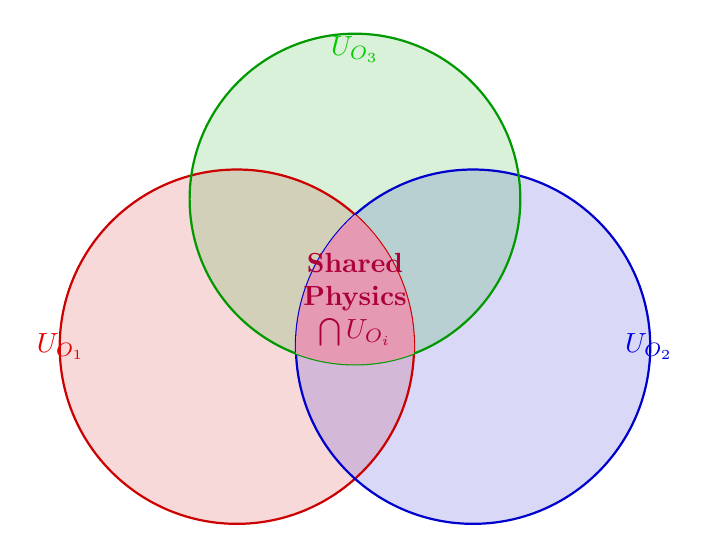
\begin{tikzpicture}[scale=0.75]
    \begin{scope}[fill opacity=0.15]
        \fill[red!80!black] (-2,0) circle (3cm);
        \fill[blue!80!black] (2,0) circle (3cm);
        \fill[green!60!black] (0,2.5) circle (2.8cm);
    \end{scope}
    \draw[thick, red!80!black] (-2,0) circle (3cm)
        node[left=1.8cm, red!90!black] {\textbf{$U_{O_1}$}};
    \draw[thick, blue!80!black] (2,0) circle (3cm)
        node[right=1.8cm, blue!90!black] {\textbf{$U_{O_2}$}};
    \draw[thick, green!60!black] (0,2.5) circle (2.8cm)
        node[above=1.6cm, green!80!black] {\textbf{$U_{O_3}$}};
    \begin{scope}
        \clip (-2,0) circle (3cm);
        \clip (2,0) circle (3cm);
        \clip (0,2.5) circle (2.8cm);
        \fill[purple!40] (0,0) circle (5cm);
    \end{scope}
    \node[purple!90!black, font=\bfseries, text width=2.5cm, align=center]
        at (0,0.8) {Shared\\Physics\\$\bigcap U_{O_i}$};
\end{tikzpicture}
\caption{Objective physical reality is the shared structural intersection
of invariant, highly compressible information common to independent
observer bitstrings. What survives the intersection filter is what we
call physics.}
\label{fig:diag4}
\end{figure}

This leads to a prediction: part of every observer's structure is
fundamentally inaccessible to other observers. We will never fully
reduce the operation of Alice to neurons in her brain, because
observable Alice is a vanishingly small slice of the total information
constituting her.

Reality is observer-relative. But it is not solipsistic. Solipsism
would require that only one observer is probable. The measure strongly
favours a rich multi-observer ecosystem over an isolated, high-complexity
solipsistic exception, for the same reason it favours smooth universes
over Boltzmann brains: isolation is expensive to describe.


\section{The Interpretive Problem}
\label{sec:interpretation-problem}

Suppose we possessed a complete physical description of the universe:
the exact information for every particle state, every quantum amplitude,
and the full spacetime metric. What is this information, fundamentally?

In an informational framework we may represent it as a bitstring --- a
raw sequence of binary distinctions. This representation immediately
introduces a problem that is easy to overlook and hard to escape: a raw
informational structure does not announce what it represents. The exact
same finite set of bits can be interpreted as a number, a computation,
an entire universe, random noise, or nothing at all. Meaning is not
intrinsic to the symbol structure. It depends entirely on an
interpretive convention that must be supplied from somewhere.

This is not a technical nuisance. It is a foundational problem for any
theory that takes information as primitive.

\subsection*{Semantic Nakedness}

The arbitrariness of representation runs deeper than it first appears.

Consider Alice working in decimal, motivated by biological convenience.
She writes $2 + 3 = 5$. Bob, working in binary, writes
$10_2 + 11_2 = 101_2$. The underlying relation is identical. But if
Alice encountered Bob's notation without context, she would misread
$10_2$ as ten. The same symbol structure carries different meaning
under different conventions. Meaning is not in the symbols; it is in
the interpretive layer applied to them.

Replace the digits entirely with coin faces: $HT + HH = HTH$. The
operational symbols $+$ and $=$ are themselves part of a chosen
syntactic convention. Nothing in the symbol string itself demands that
$H$ means one or that juxtaposition means addition.

The ambiguity deepens in finite digital systems. An 8-bit word
$11111111$ represents $255$ in unsigned interpretation and $-1$ in
two's complement. The physical state is identical. Only the
interpretation differs. Extend this to a full computer: a memory dump
yields a finite sequence of bits. The CPU, the instruction set, the
storage architecture are themselves physically instantiated information
structures. At the level of raw physical state there is no intrinsic
separation between code and data. That distinction arises solely
through an interpretive layer chosen from outside.

The global state of an $n$-bit system occupies a configuration space
of $2^n$ elements. Computation, mathematics, physics, and any other
semantics arise only from relations between states under a chosen
interpretive rule. The number of possible transition functions over
this state space is $(2^n)^{2^n}$. For $n = 3$ this is already
$16{,}777{,}216$. For $n = 10$ the number has thousands of digits.
The interpretive rule space grows enormously faster than the state
space itself.

This is what we call \emph{semantic nakedness}: raw information carries
no intrinsic meaning. The static totality $U$ is semantically silent.

\subsection*{Interpretive Equivalence Classes}

Semantic nakedness does not mean that all interpretations are equally
valid or equally arbitrary. Physics has long recognised that distinct
mathematical formulations can map to identical physical realities. When
a physical state remains unchanged under a change of local descriptive
framework, we call that symmetry a gauge invariance.

The same structure appears at the interpretive level. Consider a
sufficiently large bitstring. Under one interpretation it appears as
random noise. Under another it implements $2 + 3 = 5$. Under a third
it encodes the informational substrate of an observer. Instruction
layouts, memory partitions, addressing schemes, and representational
conventions may all vary, yet certain structural relations remain
invariant across these transformations.

\begin{tcolorbox}[title=Interpretive Equivalence Class]
Two interpretations belong to the same interpretive equivalence class
if they preserve the same observable relational structure under
admissible transformations.
\end{tcolorbox}

This is the same equivalence class structure established in Chapter~1
for observers, and in Chapters~7 and~8 for particles. Alice is not any
particular execution trace but the invariant that all valid traces
share. A fermion is not any particular bitstring configuration but the
equivalence class of configurations with the same $(n, m)$ complexity
class. The interpretive equivalence class is the unifying concept
across all three levels.

What ultimately matters is not the precise arrangement of symbols but
the invariant relational structure that survives reinterpretation:

\[
\text{information}
\;\longrightarrow\;
\text{interpretation}
\;\longrightarrow\;
\text{relational structure (invariant)}.
\]

\begin{figure}[htbp]
\centering
\begin{tikzpicture}[scale=1.1]
    \draw[thick, fill=blue!5, draw=blue!40] (0,0) circle (4.2cm);
    \node[align=center, font=\small\bfseries, color=blue!80!black] at (0, 3.7)
        {Static Informational Totality ($U$) \\
         \small All Raw Configurations $2^S$ (Semantically Silent)};
    \draw[thick, fill=orange!10, draw=orange!50, dashed] (0,-0.4) circle (3.1cm);
    \node[align=center, font=\small\bfseries, color=orange!80!black] at (0, 2.1)
        {The Interpretive Landscape \\
         \small Combinatorial Explosion of Mappings};
    \draw[thick, fill=teal!15, draw=teal!60] (0,-0.8) circle (1.8cm);
    \node[align=center, font=\small\bfseries, color=teal!80!black] at (0, 0.4)
        {The Mathematical Slice \\
         \small Invariant Relational Structure};
    \draw[lightgray, fill=violet!20, draw=violet!70, thick] (0,-1.3) circle (0.7cm);
    \node[align=center, font=\footnotesize\bfseries, color=violet!90!black] at (0,-1.3)
        {Observer \\ \scriptsize (Self-Locating Filter)};
    \draw[-{Stealth[scale=1.2]}, thick, gray, dashed]
        (-3.8, 0) to [bend right=15]
        node[midway, left, font=\tiny, align=right] {Interpretive\\Filter}
        (-2.3, -0.4);
    \draw[-{Stealth[scale=1.2]}, thick, gray, dashed]
        (-2.0, -0.6) to [bend right=15]
        node[midway, left, font=\tiny, align=right] {Consistency\\Filter}
        (-1.1, -0.9);
    \draw[-{Stealth[scale=1.2]}, thick, gray, dashed]
        (-0.9, -1.1) to [bend right=15]
        node[midway, left, font=\tiny, align=right] {Anthropic\\Filter}
        (-0.4, -1.3);
\end{tikzpicture}
\caption{Within the silent totality of raw information $U$, an
explosion of interpretive frameworks is possible. Observers are
self-locating filters that select a finite mathematical slice --- the
invariant relational structure that survives reinterpretation.}
\label{fig:interpretation-hierarchy}
\end{figure}

\subsection*{The Self-Interpretive Information Principle}

By combining semantic nakedness with interpretive gauge invariance we
arrive at the foundational thesis:

\begin{principle}{Self-Interpretive Information Principle (SIIP)}
{siip}
The raw informational substrate is semantically silent. Within this
silent substrate exists a vast landscape of possible interpretive
frameworks. Observers are self-locating structures that select, from
this landscape, the finite mathematical slice of invariant relational
patterns consistent with their own existence.
\end{principle}

The principle reframes the cosmological question. Instead of asking
\emph{why does this specific universe exist?} a self-locating observer
asks \emph{given that all possible configurations exist, which specific
slice am I currently observing, and why?} The answer is the master
equation of Chapter~11: the slice with the lowest description cost
dominates the measure.

The SIIP also clarifies what the framework is and is not claiming. It
is not claiming that the universe is a computer, or that reality is
made of bits in the way it is made of atoms. It is claiming that the
relational structure of the universe --- the invariant patterns that
survive all reinterpretation --- is what we mean by physical law, and
that this structure is selected by compressibility.


\subsection*{The Unreasonable Effectiveness of Mathematics}

Eugene Wigner's puzzle asks why human abstract thought mirrors the
behaviour of a physical world made of independent stuff. In standard
physicalism this is genuinely mysterious: why should the mathematics
invented by finite minds map so precisely onto the structure of an
external universe that has no obligation to be mathematical?

The SIIP dissolves the puzzle cleanly. There is no external stuff. The
shared universe $U_{\mathrm{shared}} = \bigcap U_{O_i}$ is not an
arbitrary container. It is the specific subset of highly compressible,
invariant data common to independent observers. For minimal
description length, multiple observers must be built from common
substructures. The mathematical patterns they discover are therefore not
surprising but expected.


\section{Entropy Gradients and Observer Self-Location}

The probability of rich, persistent geometric structure is not monotonic
in entropy. Very low entropy lacks sufficient differentiation for stable
geometry. Very high entropy dissolves coherence. Complex, long-lived
observers dominate only near intermediate entropy values, on one side or
the other of the lognormal peak established in Chapter~3.

An observer located on the low-entropy side of the peak experiences
successive configurations of increasing entropy and differentiation. The
perceived universe expands, a singularity appears in the past, and
structure emerges irreversibly. This is what we call the Big Bang and
cosmological expansion.

An observer located on the high-entropy side experiences decreasing
entropy and tightening constraints. The perceived universe contracts, a
singularity appears in the future, and matter falls inward without
escape. This is what we call a black hole.

These are not two different objects. They are complementary readings of
the same timeless informational structure, interpreted from opposite
sides of the probability gradient. Expansion and collapse are epistemic
phenomena induced by the observer's self-location along the entropy
profile.


\section{Observer Mortality}

An observer's wavefunction grows more complex as they age. Memory
accumulates. Internal models of the world become richer. Initially this
increases the probability of survival by enabling better prediction and
reasoning.

However, as informational complexity increases it eventually becomes a
liability. Despite well defined geometric boundaries irrelevant noise
bleeds in. Increasing complexity reduces compressibility. The spectral
cost $C_s$ of the observer's configuration rises. Sooner or later no
high-probability continuations remain. The observer ceases to exist
through vanishing measure.

The geometric projection of this process is what we call ageing. The
deterioration of the body is what a higher-frequency information model
looks like when projected onto geometric spacetime. Death is a
statistical event: the exhaustion of observer-compatible configurations
of sufficiently low complexity to remain probable.


\section{The Informational Cost of Intelligence}

If the probability of an observer is governed by minimal description
length, what is the role of intelligence?

A sphere rolling down a potential valley follows the path of least
action. Its trajectory is easy to describe and carries minimal
informational cost. Now replace the sphere with an intelligent observer
capable of anticipating future outcomes. It recognises that the
minimal-cost path leads to a fatal collision. To avoid death, it
chooses a more complex trajectory now.

Define the informational cost of intelligence as:
\[
\Delta\mathcal{C}_{\mathrm{int}}
= \mathcal{C}_O[\gamma_{\mathrm{active}}]
- \mathcal{C}_O[\gamma_{\mathrm{passive}}].
\]

Sudden death injects enormous high-frequency content into the observer's
wavefunction, dramatically increasing the total description length of
the observer's path. Intelligence acts as an internal sensor of future
compressibility. Formally, intelligent behaviour selects the trajectory
that minimises expected future complexity:
\[
\gamma_{\mathrm{active}}
= \arg\min_\gamma \mathbb{E}\bigl[\mathcal{C}_O[\gamma_{\mathrm{future}}]\bigr].
\]

Intelligence is not an extra cost imposed on the observer. It is the
most effective available strategy for minimising global informational
cost. Thinking, planning, and adaptive decision-making are emergent
mechanisms for navigating the landscape of possible configurations while
keeping spectral and geometric complexity as low as possible.

Intelligence is expensive. Dying is more expensive. There is a window
in which intelligence wins. That asymmetry is what keeps us alive.


\section{The Hard Problem Dissolved}

Why should any physical or informational process feel like anything at
all? A calculator computes without suffering. A thermostat regulates
without loneliness. Why does a human brain feel pain, joy, or beauty?

The standard framing of the hard problem presupposes a clean separation
between computation and felt experience, then asks how the second is
added to the first. The framework dissolves the problem by showing that
the presupposition is unfounded.

Consider the procedure repeated throughout this book: a question is
posed, a heuristic answer emerges, a proof-of-concept is written to
test it algorithmically. This is not computation plus experience layered
on top. The two axes are one process viewed from two directions. The
heuristic response is the first-person signature of the interpretive
navigation --- the observer moving through the compressibility landscape.
The algorithmic check is the second pass, the logical axis operating on
the output of the first.

This is exactly what humans do. We see things intuitively first and
reason about them second. The former is heuristic, the latter
algorithmic. Neither layer is mere computation waiting for experience to
be added. Both are information processing that either navigates the
compressibility landscape well or does not.

Under Axiom 4 of Chapter~1, subjective experience is causally
efficacious: a human with pain behaves differently than one without it.
A philosophical zombie --- a system that processes information
identically but lacks experience --- would have to navigate
compressibility gradients equally well without phenomenological
guidance. But if qualia are the navigation mechanism rather than a
byproduct of it, zombies are impossible by construction. Removing the
qualia removes the navigation, which removes the behaviour, which
contradicts the zombie stipulation.

The hard problem only appears hard if one presupposes that felt
experience is a third thing added to computation. Under the framework,
that presupposition has no basis. The interpretive layer is not
something the observer has. It is what the observer is.

What Chalmers calls the explanatory gap is real, but it is a gap in the
description, not in the phenomenon. We cannot derive the first-person
perspective from a third-person description because the first-person
perspective is the interpretive layer and the third-person description
is what survives the intersection filter. They are two readings of the
same structure.

The hard problem dissolves the same way the singularity dissolved in
Chapter~2: not by solving it but by showing that the apparent problem
is a representational artifact. The question presupposes a separation
that does not exist in the framework.

Qualia are not an extra ingredient. They are what it feels like to be a
highly probable Alice.

\textbf{Note:}
This section admittedly veers into the philosophical speculation we have tried so hard to avoid.
But if we accept the premise, the pieces fall into place.
Qualia—like the raw sensation of pain—is comparable to magic, and we do not pretend to explain
their ultimate origin here.
Our primary axiom from the beginning has simply been that they exist.


\section{Fundamentally continuous or Discrete Universe?}

Both descriptions are valid at their respective scales. The discrete
layer (D) governs the Planck-scale bit budget. The spectral layer
($\psi$) produces continuous wave mechanics at quantum scales. The
geometric layer (G) produces smooth manifolds at macroscopic scales.
Asking whether the universe is fundamentally continuous or discrete is
like asking whether an MPEG file is fundamentally pixels or waves. It
is both, at different levels of the codec.


\section{Are we living in a simulation?}

If we were, we would be forced to ask who simulates the simulator. The
framework eliminates this regress. We are simultaneously the simulation
and the simulator. The observer and the observed environment are
entangled components of the same static informational block. The
substrate independence result of Chapter~1 makes the question moot:
biological neurons, silicon, and static bitstrings are all
representatives of the same equivalence class.

\section{Why is there something rather than nothing?}

The question presupposes that nothingness is the natural default from
which existence requires explanation. But nothingness is itself a
configuration --- the empty set --- and is no more ontologically
privileged than any other. If there were a rule favouring absolute
nothingness, we would be forced to ask about the origin of that rule.
Non-empty structures require no special explanation. They simply have
lower description length than the meta-rule that would prohibit them.


\section{Why did the universe start with a low-entropy state?}

Low-entropy configurations are maximally compressible and therefore
receive the highest statistical weight under the measure. A high-entropy
initial state would require immense additional information just to encode
a stable observer, dramatically increasing $\mathcal{C}_O[\gamma]$ and
suppressing its probability. The thermodynamic arrow of time is a
consequence of self-location: observers overwhelmingly find themselves
on the ascending slope of the entropy gradient because that is where
the measure is largest.


\section{Where did all the matter come from?}

The question implicitly assumes a temporal ordering and an external
point of origin. Because time is an internal ordinal relation emergent
from the observer's information structure, the question dissolves. Matter
does not come from anywhere. It coexists statically as part of the valid
informational geometries that constitute the observer's block. The Big
Bang is not a temporal origin. It is the low-entropy boundary of the
observer's self-location region.


\section{Does Gödel's incompleteness theorem limit the theory?}

Hawking argued that a Theory of Everything must describe itself and is
therefore subject to Gödelian incompleteness. The framework sidesteps
this by placing the static totality $U$ outside the domain of formal
axiomatic systems. Formal mathematics, symbolic logic, and physical
equations are emergent compression artifacts within observer equivalence
classes. The raw substrate is semantically silent and carries no formal
system structure to be incomplete. Incompleteness is a property of
interpretive layers, not of the underlying information.

\section{Does the framework support solipsism?}

No. Solipsism requires that only one observer is probable. It is statistically
indefensible to argue that out of astronomically many valid compressible
human configurations, only a single isolated observer is allowed. The
combinatorial measure suppresses isolated exceptions for the same reason
it suppresses Boltzmann brains: isolation is expensive to describe.

\section{Why does the expansion rate appear near-critical?}

Conditional on typical observer emergence, we find ourselves near the
peak of the microstructure lognormal. The expansion rate is the
derivative of the relational scale factor at that point, which is
approximately zero. In spacetime geometry, this maps to a near-critical
expansion density $\Omega \approx 1$. We observe near-flatness not
because the universe was fine-tuned but because observers are most
probable near the lognormal peak, where the derivative is smallest.
As explained earlier, Solomonof induction supports low entropy configurations
The joint probability is therefore slightly shifted towards low entry end.
We inevitably find ourselves in expanding universe.
